\documentclass{ecnreport}

\stud{EMARO-ARIA ROBA M2}
\topic{Sensor-based control}

\begin{document}

\inserttitle{Sensor-based control lab}

\insertsubtitle{Labs 3: Multi-sensor control with constraints}



\section{Content of this lab}

The goal is this lab is to control a mobile robot equipped with a pan-tilt camera 
 (see \Fig{fig:vrep}).

\begin{figure}[h!]\centering
 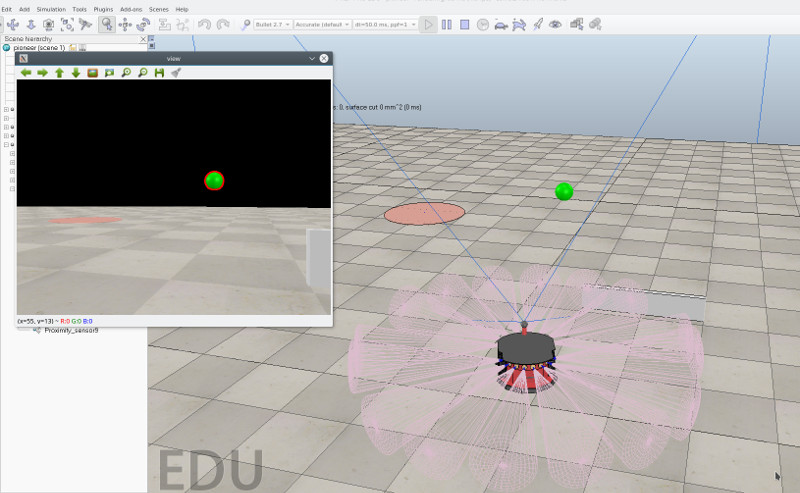
\includegraphics[width=.8\linewidth]{vrep}
 \caption{V-REP simulator with the mobile robot, image from the onboard camera and US sensors.}
 \label{fig:vrep}
\end{figure}

The robot is simulated with V-REP\footnote{Virtual robot experimentation platform, http://www.coppeliarobotics.com/}.
In the simulation are placed a green sphere and a target. The goal of the robot is to move to the target position while maintaining visibility on the sphere.
The robot control will be performed in C++ and will rely on:

\begin{itemize}
 \item The ROS framework to handle communication between the simulator and the control program.
 \item The ViSP library\footnote{Visual Servoing Platform, http://visp.inria.fr} to manipulate vectors and matrices and to perform linear algebra.
\end{itemize}
The actual classes that are used are detailed in Appendix \ref{sec:classes}.\\

\subsection{Environment setup}

To use this lab (and for some other ROS labs) you need to initialize the ROS environment in order to have access to the ViSP library.
To do so, download the following file and execute it:
\begin{center}\cppstyle
\begin{lstlisting}
        wget http://www.irccyn.ec-nantes.fr/~kermorga/files/ros_user_setup.sh
        sh ros_user_setup.sh
\end{lstlisting}
\end{center}In order to use an IDE like Qt Creator, you should open a new terminal and launch the IDE from the command line.\\

This lab is available on GitHub as a ROS package called \texttt{ecn\_sensorbased}. In order to download it, you should first go in the \texttt{ros/src} directory. The package can then be downloaded through git:
\begin{center}\cppstyle
\begin{lstlisting}
 git clone https://github.com/oKermorgant/ecn_sensorbased.git
\end{lstlisting}
\end{center}

\subsection{Structure of the \texttt{ecn\_sensorbased} ROS package}

The package has the classical ROS structure:
\begin{figure}[h]
\begin{minipage}{.25\linewidth} ~ \end{minipage}
\begin{minipage}{.5\linewidth}
 \dirtree{%
.1 ecn\_sensorbased. 
.2 include.
.3 ecn\_sensorbased. 
.4 pioneer\_cam.h.
.4 qp.h.
.4 utils.h.
.2 launch.
.3 us\_config.yaml.
.3 vrep.launch.
.2 scenes.
.3 pioneer.ttt.
.2 scripts.
.3 check\_vitals.py.
.2 src.
.3 main.cpp.
.3 pioneer\_cam.cpp.
.2 subject.
.2 package.xml.
.2 CMakeLists.txt.
} 
\end{minipage}
%\begin{minipage}{.2\linewidth} ~ \end{minipage}
\caption{Files used by the package}
\end{figure}

The only file to be modified is \texttt{main.cpp}, which is the main file for the C++ program. \\
The simulation can be launched with: \texttt{roslaunch ecn\_sensorbased vrep.launch}. It will be run and stopped automatically from the main control.

When both the simulation and the control program run, the ROS graph looks like this:

\begin{figure}[h!]\centering
 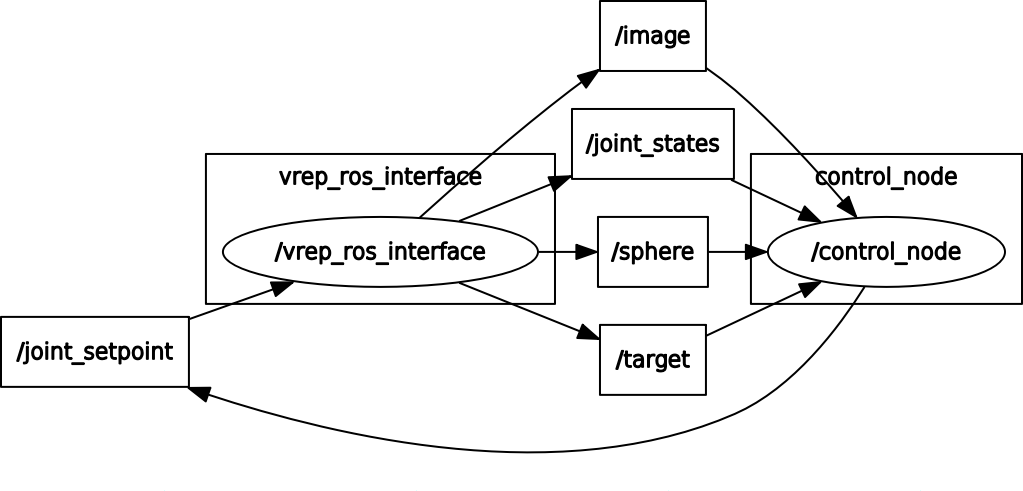
\includegraphics[width=.8\linewidth]{rosgraph}
 \caption{ROS graph showing nodes (ellipses) and communication topics (rectangles)}
 \label{fig:rosgraph}
\end{figure}

We can see that the simulator sends the joint states, camera image, target and sphere positions to the control node. In return, the control node sends the joint setpoints
to the simulator. They are velocity setpoints for the wheels and the pan-tilt camera joints.\\
The \texttt{check\_vitals} is a script that checks the control node is running and stops the simulation otherwise.


\subsection{The PioneerCam robot}

The simulated robot is a Pioneer P3dx. A pan-tilt camera is placed at the front of the robot. The robot is controlled 


\appendix

\section{Main classes}\label{sec:classes}

\subsection{ViSP classes}

This library includes many tools for linear algebra, especially for 3D transformations. 
The documentation is found here: \url{http://visp-doc.inria.fr/doxygen/visp-daily/classes.html}.\\
The main classes from ViSP (at least in this lab) are:
\begin{itemize}
\item \texttt{vpMatrix} represents a classical matrix, can then be transposed, inversed (or pseudo-inversed), multiplied with a vector, etc.
\item \texttt{vpColVector} is a column vector with classical mathematical properties.

 \subsection{The PioneerCam class}
 
 The \texttt{VVS} class implements the minimization algorithm. It is instanciated with:
 \begin{center}\cppstyle
\begin{lstlisting}
        VVS vvs(cam, d, r, c);
\end{lstlisting}
\end{center}where cam is the camera model that is used (PerspectiveCamera or DistortionCamera), d is the inter-point distances of the real landmark, and r and c are the number of rows and columns. The VVS uses these values to initialize the true position of the 3D points.

Only two methods are to be modified:
\begin{itemize}
    \item \texttt{void calibrate(std::vector<Pattern> \&\_pat)} (already quite written)\\ solves the calibration problem from a given set of \texttt{Pattern}. 
    \item \texttt{void computePose(Pattern \&\_pat, vpHomogeneousMatrix \&\_M, const bool \&\_reset)} \\ 
    solves the pose computation problem from a single \texttt{Pattern} (one image with extracted points).\\ This method can be highly inspired from the calibrate method, as shown in Section \ref{sec:pose}.
\end{itemize}

This class also have useful attributes:
\begin{itemize}
 \item \texttt{std::vector<vpPoint> X\_}: a vector of the true 3D position of the points, and is to be used in the reprojection error
 \item \texttt{GenericCamera* cam\_}: the camera that we are using or calibrating, it is a pointer to the methods can be called by using an arrow
\end{itemize}
As a syntax example, here is how we compute the (u,v) pixel coordinates of point k assuming a transformation matrix M (which can be quite useful for reprojection error):
 \begin{center}\cppstyle
\begin{lstlisting}
double u,v;
X_[k].track(M);		     // X_[k] is computed in the camera frame
cam_->project(X_[k], u, v);  // u and v are now the pixel coord. for the current camera model
\end{lstlisting}
\end{center}




\end{document}
